% This is samplepaper.tex, a sample chapter demonstrating the
% LLNCS macro package for Springer Computer Science proceedings;
% Version 2.20 of 2017/10/04
%
\documentclass[runningheads]{llncs}
%
\usepackage{graphicx}
\usepackage{makecell}
\usepackage{algorithm,algorithmic}
% Used for displaying a sample figure. If possible, figure files should
% be included in EPS format.
%
% If you use the hyperref package, please uncomment the following line
% to display URLs in blue roman font according to Springer's eBook style:
% \renewcommand\UrlFont{\color{blue}\rmfamily}

\begin{document}
%
\title{Automated verification of electrical systems: literature review and case studies of stand-alone solar photovoltaics\thanks{Supported by Newton Fund (ref. 261881580) and FAPEAM
(Amazonas State Foundation for Research Support, calls 009/2017 and PROTI Pesquisa 2018).}}
%
%\titlerunning{Abbreviated paper title}
% If the paper title is too long for the running head, you can set
% an abbreviated paper title here
%
\author{Alessandro Trindade\inst{1}\orcidID{0000-0001-8262-2919} \and
Lucas Cordeiro\inst{2}\orcidID{0000-0002-6235-4272}}
%
\authorrunning{A. Trindade and L. Cordeiro}
% First names are abbreviated in the running head.
% If there are more than two authors, 'et al.' is used.
%
\institute{Federal University of Amazonas, Av. Gen. Rodrigo Octavio, 6200, Coroado I, 69077-000 Manaus AM Brazil \email{alessandrotrindade@ufam.edu.br} \and
The University of Manchester, Kilburn Building, Oxford Road, Manchester M13 UK
\email{lucas.cordeiro@manchester.ac.uk}}
% \and ABC Institute, Rupert-Karls-University Heidelberg, Heidelberg, Germany\\
%\email{\{abc,lncs\}@uni-heidelberg.de}}
%
\maketitle              % typeset the header of the contribution
%
\begin{abstract}
Around 1 billion of people do not have electrical energy nowadays on Earth. Energy poverty alleviation has become an important political issue. Several initiatives and policies have been proposed to deal with poor access to sources of energy in many developing countries. Particular attention is given to use renewables and stand-alone solar photovoltaic systems. Tools to evaluate electrification projects are available, but they are based on simulations that do not cover all aspects of the design space. The use of automated verification in electrical systems is a fresh subject with few issued literature. This paper do a state-of-art review about the use of automated verification on electrical systems and perform a comparative of tolls applied to five stand-alone solar photovoltaic systems. Information about the use of a commercial simulator and monitoring data from the deployed systems are used to validate the research. Data from experimental results shows that only some flaws can be detected by automated verification and that ESBMC verification engine obtain the best results, regardless using a high-end or low-end setup.

\keywords{Automated verification  \and Model Checking \and Electrical systems \and Solar photovoltaic systems.}
\end{abstract}
%
%
%
\section{Introduction}
%%%%%In 2015, 193 Member States of the United Nations agreed as part of the Sustainable Development Goals (SDG) with a specific target to 'ensure access to affordable, reliable and modern energy for all by 2030' – universal access to electricity and clean cooking~\cite{IEAeao2017}. Therefore electricity has a important role, based on two main issues: %that are on the agenda of all current rulers and society in general, regardless of whether it is a developed, emerging or developing country: 
%%%%%the impact on the global climate change and poverty alleviation.
%
%%%%%Related to climate change, the 23rd session of the Conference of the Parties (COP23) to the United Nations Framework Convention on Climate Change (UNFCCC) in 2017 was the second session after the Paris Agreement, which aims to keep the maximum global average temperature rise as close as possible to 1.5 $^{o}$C. %During COP23, with respect to the future market development of renewable power and solar PV (photovoltaics) in particular, it was created an alliance of nations and states committed to moving the world from burning coal to cleaner power sources was a promising sign at COP23 \cite{Jager-Waldau}. 
%%%%%Decarbonization of our energy supply is an important component to achieve the targets, because 65.3\% of the worlds current CO\textsubscript{2} emissions (from energy supple) are due to burning fossil fuels according with 2016 data: 81.1\% of our total primary energy supply depended on burning fossil fuels, namely 27.1\% coal, 31.9\% oil and 22.1\% natural gas~\cite{IEAwes2018}. In terms of final energy consumption electricity only accounted for 18.6\%, but was responsible for 32\% of the total CO\textsubscript{2} emissions~\cite{IEAwes2018}. Photovoltaics (PV) is one of the key technology options for implementing the shift to a decarbonized energy supply, because it is abundant, cannot be monopolized  and can be deployed in a modular way almost everywhere on Earth.
%
%Related to poverty alleviation, 
%
%In reality, the biggest barrier to universal energy access is not the capacity to generate electricity, but rather the ability to get energy to those who need it most. The concept of energy poverty and access tends to focus on very small, incremental shifts in the delivery of energy to poor people. The total energy demand of these shifts constitutes only a small fraction of the ‘gap’ between electricity supply in much of Africa versus more industrialised countries, or the gap between the region’s current and projected electricity supply. https://policy-practice.oxfamamerica.org/static/media/files/FINAL_speakingpowertotruth_SH.pdf
%
%%%%%Poverty, in other hand, needs to be addressed through socio-economic development. Poverty %is conceptualized in material terms as not having access to adequate levels of food, water, clothing, shelter, sanitation, health care and education. This 
%%%%%can be translated into people having insufficient income. 
%
For numerous people around the world, a better life means getting access to basic needs such as food, health services, housing and clean water. None of these basic needs can be provided without energy. Energy is one of the most essential inputs into sustaining people‘s livelihoods. Lack of access to clean and affordable energy is considered a core dimension of poverty~\cite{Hussein2012}. 

Progress has been made worldwide. The number of people without electricity access fell below 1 billion for the first time in 2017~\cite{IEAweo2018}. To provide universal electricity for all, decentralized systems, led by solar PV in off-grid and mini-grid systems, will be the least-cost solution for three-quarters of the additional connections needed, but that grid extension will still have a role to play, especially in urban areas~\cite{IEAweo2018}.

%With worldwide over 400GW cumulative installed photovoltaic electricity generation capacity installed by the end of 2017, photovoltaics still is a small contributor to the electricity supply with a little of 2\%, but its importance for our future energy mix is now acknowledged and with the fastest growth (32\% whem compared with 2016 numbers)~\cite{Jager-Waldau}.
%
In order to simulate or evaluate a PV system there are a myriad of specialized tools available in the market, such as RETScreen, HOMER, PVWatts, SAM, and Hybrid2 \cite{Pradhan,Swarnkar,NRELDobos,NRELBlair,Mills}; and even general purpose simulation tools such as PSpice, Saber, or MATLAB/Simulink package \cite{Gow1999,Benatiallah2017}. However, those tools are based on running experiments in simulation models. Simulation %has the advantage of being cheap (if compared to test in real systems) and can be 
is employed before the system design is concluded but it has the drawback of an incomplete coverage since the verification of all possible combinations and potential failures of a system is unfeasible~\cite{ClarkeHV18}.

Formal methods based on model checking offer a great potential to obtain a more effective and faster verification in the design process~\cite{ClarkeHV18}. Any kind of system can be specified as computer programs using mathematical logic, which constitutes the intended (correct) behavior; then, one can try to give a formal proof or otherwise establish that the program meets its specification. 

In this study, an updated review about the use of verification tools in electrical systems is performed, and is presented five case studies, where different model checking tools are compared in terms of performance and reliability when validating stand-alone solar PV systems. In order to perform the comparation and case studies, a mathematical model of each component of a stand-alone PV system, as panel solar, charge controller, batteries, inverter, and electrical load is used. The project requirements, as battery autonomy and power demand, besides weather conditions, as solar irradiance and ambient temperature, are translated as part of the computer program and automatically verified during the formal process. The model checking tools report in which conditions a system does not meet the user requirements. A key benefit to this approach is that it helps in the detection of flaws in the design phase of system development, thereby considerably improving system reliability~\cite{Akram2018}. The case studies are not theoretical and were deployed in 2018, with feedback information collected from monitoring systems and through interview with the dwellers. 
%The implementation of the proposed tool is carried out by means of the efficient SMT-based bounded model checker (ESBMC)~\cite{esbmc2018}.
\section{State-of-art in automated verification of Electrical systems}
This section summarizes, in a chronological way, the research done by previous studies related to the subject of this research.

The conversion of traditional power grid into a smart grid, a fundamental example of a cyber-physical system, raises a number of issues that require novel methods and applications. In 2012, it was considered a specific Chinese Smart Grid implementation as a case study and address the verification problem for performance and energy consumption~\cite{Yukseletall2012}. It was employed the stochastic model checking approach and present a modelling and analysis study using PRISM model checker. The focus was how Cyber-physical systems integrate information and communication technology functions to the physical elements of a system for monitoring and controlling purposes.  In this context, it was applied automated verification of certain quantitative properties of the system. %, with no interest in power generation or even solar PV systems.

%In 2014, there were a research showing that power systems model information exchange and the simulation of user defined models is a challenge issue for the transmission system operator. The reason: the use of different simulation software with specific data format and models strongly coupled to the simulation software numerical routines. The researchers proposed the use of Open Source software (Modelica, JAVA and Python) for simulation and modelling as a solution to decouple these models. The work described the design of a simulation tool following the Free/Libre Open Source Software philosophy to simulate equation-based models and implement a standard data format for model information exchange~\cite{Gomez2014}. The aim was the use of Modelica to define standards and industry models, besides the interest of components in modules. This work did not reached the automated verification, it is just simulation, however created the base to future work of formal methods on electrical systems.
%
In 2015, it was showed that related to power system protection schemes, the approach of using Monte-Carlo simulation and manual interpretation of results had the limitation of the incomplete coverage of all possible operating conditions due to the time complexity of simulation~\cite{Sengupta2015}. It was proposed an automated simulation-based verification technique to verify the correctness of protection settings efficiently using hybrid automata-temporal-logic framework. The initial focus were relay operations and test-case generation to ensure early detection of design errors. %The study was limited to power system protection and did not deal with electricity generation or even solar PV systems.

Other work issued in 2015 was a framework named Modana to achieve an integrated process from modeling with SysML/MARTE to analysis with Statistical Model Checking (SMC) for Cyber-Physical Systems (CPSs) in terms of Non Functional Properties (NFP) such as time, energy, etc~\cite{Cheng2015}. To demonstrate the capability of Modana framework, the authors modelled energy-aware buildings as a case study, and discussed the analysis on energy consumption in different scenarios. The focus is in smart buildings and HVAC (Heating, ventilation, and air conditioning) systems. %The research did no deal with solar PV systems. 
 
Back in 2017, it was suggested the use of formal methods to verify and certifiably control the behavior of computational devices interacting over a shared and smart infrastructure~\cite{Abate2017}. It was shown that formal techniques can provide compelling solutions not only when safety-critical goals are the target, but also to tackle verification and synthesis problems on populations of such devices. This work argued that alternative solutions based on classical analytical techniques or on approximate computations are prone to errors with global repercussions. Two different areas were targeted: thermal loads and electricity-generating devices interacting over a smart energy network or over a local power grid. The researcher discussed the aggregation of large populations of thermostatically-controlled loads and of photovoltaic panels, and the corresponding problems of energy management in smart buildings, of demand-response on smart grids, and respectively of frequency stabilization and grid robustness. The focus is in controlling the behavior of the components, verifying the smart grid, dealing with a 'system of systems' and with 'internet of things'. The author uses approximate model checking of stochastic and hybrid models. % Therefore, the focus is not in electricity generation or even the components of a stand-alone solar PV system.

In 2018, is was proposed a methodology for the verification of the Cyber Physical Energy Systems (CPES), with the methodology applied to PV panels and its distributed power point tracking~\cite{Driouich2018}. The approach relied on representing the unpredictable behavior of the environment in order to cover all feasible possible scenarios. Processed by JModelica, the simulation results covered the system's complete dynamic behavior. It was evident at this work the time consuming issue, with almost three days of computer effort to verify the design space of one hour from PV panels behavior. %The work did not include the other components of a stand-alone solar PV system.

Another work issued in 2018 was the approach to modeling smart grid components using a formal specification. It was used a state-based formal specification language namely Z %(pronounced as `Zed') 
and it was demonstrated the application of Z on four smart grid components~\cite{Akram2018}. The presented formal specification can be considered as first steps towards modeling of smart grid using a Software Engineering formalism. The starting point of this work it was that a smart home can be considered as an integrated system consists of various objects and system, that communicates and interact  with  each  other. The approach is base in Petri nets and from the premise that modeling of the smart home leads to clear understanding the overall behavior of the smart grid.

\section{Automated Verification Using Model Checking}
\label{sec:AutomatedVerification}
%--------------------------------------------------
%It is necessary to keep in mind that 
Validation is the process of determining whether a design meets the user requirements, whereas verification is the process of determining whether a design meets a set of requirements, specifications, and regulations~\cite{ClarkeHV18}. If the requirements, specifications, and regulations are given in a formal language, then it may be possible to automate the verification process, thus resulting in a process known as \textit{formal verification}. Verification may form part of a validation process.
%, but in general, validation cannot be formalized because it relates a system design to intent.  
While simulation and testing explore some of the possible behaviors and scenarios of the system, leaving open the question of whether the unexplored trajectories may contain a flaw, formal verification conducts an exhaustive exploration of all possible behaviors. Thus, when a design is pronounced correct by a formal verification method, it implies that all behaviors have been explored, and the questions of adequate coverage or a missed behavior becomes irrelevant \cite{Clarke2012}.
%Simulation may also be used for validation, but it is more problematic for verification.
%In order to use simulation for verification, it is necessary to ensure adequate coverage of operating conditions, scenarios, and system inputs. Testing can also be used for validation, however it is not feasible to cover all the aspects of the design space, and some times the real system must be used instead of a computing model.
 %

Formal verification is a systematic approach that applies mathematical reasoning to obtain guarantees about the correctness of a system; one successful method in this domain is model checking \cite{Clarke2012}.
%%%%%%%%Formal verification is a systematic approach that applies mathematical reasoning to obtain guarantees about the correctness of a system \cite{Forejt2011}; one successful method in this domain is model checking \cite{Clarke2012}.

% 
%Model checking is an automatic verification technique, as defined by \cite{ClarkeHV18}. Model checking was originally developed reasoned about finite state of concurrent systems, nowadays is mainly used to hardware and software verification, but can be applied to any kind of system. 
%
The process of model checking can be split into three main components: modeling, specification, and verification method. In modeling, a model (normally mathematical) of the system is created; in specification, normally a list of properties to be satisfied by the system is established, i.e., the requirements, normally  expressed in a temporal logic form as Computational Tree Logic (CTL) or Linear Temporal Logic (LTL).
%
%\begin{itemize}
%\item In modeling, a model (normally mathematical) of the system is created; 
%\item In specification, normally a list of properties to be satisfied by the system is established, i.e., the requirements, as reliability to performance for example. \item Normally is expressed in temporal logic form ($CTL$); 
%\item The model checking is the verification method itself. 
%\end{itemize}
%
%%%%%
%%%%%The model checking algorithm can be described as \cite{ClarkeHV18}:  (i) Given the model $M$ and a CTL (or LTL) formula $ \phi $ as input;  (ii) Model checking algorithm provides all the states of model $ M $ which satisfies $ \phi $;  and (iii) It returns \textit{YES} if $ \phi $ is \textit{TRUE}, or returns \textit{NO} if $ \phi $ is \textit{FALSE}. Specifically for the \textit{FALSE} verification result, the algorithm returns a \textit{counterexample} (i.e., a sequence of states that leads to a property violation), which is useful as diagnostic of the system to discover in which situation the model is violated; this is the most important advantage of the use of model checking~\cite{ClarkeHV18}. 
%%%%%
%%%%%%%%%%%%%%%Fig.~\ref{fig:systemverif} shows a real PV system, and Fig.~\ref{fig:systemverif2} the conversion the system to be verified by a model checking procedure. % \textcolor{red}{Please try to adapt this figure to our context. How can it be applied to verify PV?}. 
%Fig.~\ref{fig:systemverif} shows the process to convert a real PV system to a model to be verified by a model checking procedure. % \textcolor{red}{Please try to adapt this figure to our context. How can it be applied to verify PV?}. 
%
%\begin{figure}[h]
%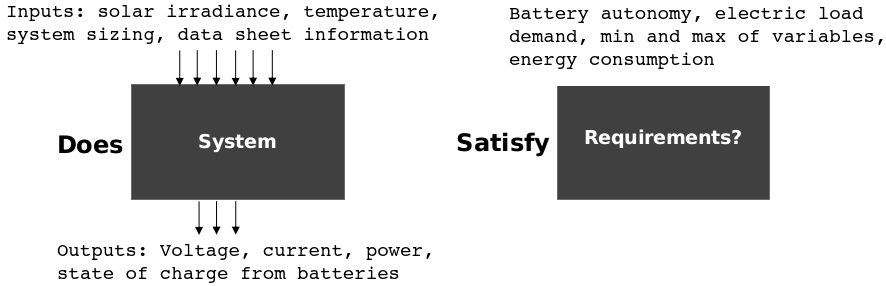
\includegraphics[width=0.5\textwidth]{system_original_blocks}
%\centering
%\caption{Real system verification (adapted from \cite{ClarkeHV18}).}
%\label{fig:systemverif}
%\end{figure}
%
%\begin{figure}[h]
%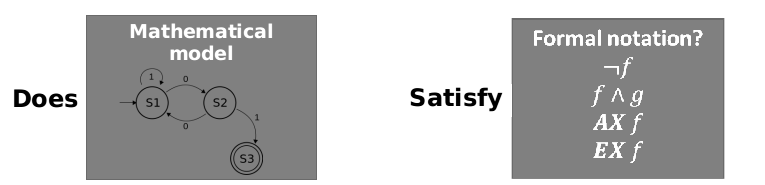
\includegraphics[width=0.4\textwidth]{system_model_blocks}
%\centering
%\caption{Model checking verification \cite{ClarkeHV18}.}
%\label{fig:systemverif2}
%\end{figure}
%
However, there is a main disadvantage of model checking: the state explosion problem. In order to tackle this problem, many different techniques were developed in the last decades. One of the first major advances was symbolic model checking with binary decision diagrams (BDDs). In this approach, a set of states is represented by a BDD instead of by listing each state individually, which is often exponentially smaller in practice.
% Another major advance is the partial order reduction, which exploits the independence of actions in a system with asynchronous composition of processes \textcolor{red}{add citation here}. A third major advance is counterexample-guided abstraction refinement, which adaptively tries to find an appropriate level of refinement, not burdened with irrelevant detail that slows down verification \cite{Clarke2012}. 
%
Another promising approach to overcome state explosion problem is Bounded Model Checking (BMC)~\cite{DBLP:conf/tacas/BiereCCZ99}. BMC is a method that checks a model up to a given path in the path length. BMC algorithms traverse a finite state machine for a fixed number of steps, $ k $, and checks whether a property violation occurs with this bound. It uses Boolean Satisfiability (SAT) or Satisfiability Module Theories (SMT) solvers to check the generated formula from BMC. 

SAT problem is a problem of determining whether there are certain conditions or interpretations that satisfy a given Boolean expression \cite{ClarkeHV18}. 
SMT decides the satisfiability of a fragment of first-order formulae using a combination of different background theories and thus generalizes SAT by supporting uninterpreted functions, linear and non-linear arithmetic, bit-vectors, tuples, arrays, and other decidable first-order theories~\cite{ClarkeHV18}.
The SAT or SMT solvers search the model for conditions (value of variables) that make the formula satisfiable. If a SAT or SMT solver finds a substitution for the formula/function then the substitute induces a counterexample and is said to be \textit{satisfiable}, i.e., it is satisfiable \textit{iff} the verified system contains errors.  
%
%CBMC is considering the best-known model verification tool to validate code in ANSI-C and C++ \cite{Kroening}. 
%
%\textcolor{red}{ESBMC does not use CBMC as its main frontend. Please take a look at this paper and cite it: https://ssvlab.github.io/lucasccordeiro/papers/ase2018.pdf. I would also suggest to remove the above sentence.}
%
\subsection{CBMC}
The C Bounded Model Checker (CBMC) is considering the best-known model verification tool to validate code in ANSI-C and C++ \cite{Kroening}. CBMC demonstrates the violation of assertions in C programs, or proves safety of the assertions under a given bound.
CBMC implements a bit-precise translation of an input C program, annotated
with assertions and with loops unrolled to a given depth, into a formula. If the
formula is satisfiable, then an execution leading to a violated assertion exists~\cite{Kroening}.

CBMC's verification flow can be summarized in four stages: (i) Front-end that can read, perform parse and type checker of the C/C++ code; (ii) Intermediate Representation. CBMC uses  intermediate representation, converting all non-linear control flow, such as if or switch statements, loops and jumps, into equivalent guarded goto statements; aiming to reduce the verification effort; (iii) Middle end. CBMC performs symbolic execution by eagerly unwinding loops up to a fixed bound, which can be specified by the user on a per-loop basis or globally, for all loops and finally; (iv) Back-end. With support to SAT and SMT solvers. Conversely, if the formula is unsatisfiable, no assertion can be violated within the given unwinding bounds.
%--------------------------------------
\subsection{ESBMC}
%--------------------------------------
ESBMC (or Efficient SMT-based Bounded Model Checker) is an open source, permissively licensed (Apache 2), cross platform bounded model checking for C and C++ programs~\cite{esbmc2018}, which supports the verification of LTL properties with bounded traces~\cite{DBLP:journals/sosym/MorseCN015}. 
%The use of SMT, instead of Boolean Satisfiability SAT from the original BMC, 
ESBMC comes as an alternative to overcome limitations of the system modeling, especially considering that the system complexity is increasing and SMT has richer theories than SAT to represent models. 
%
ESBMC's verification flow can be summarized in three stages: (i) a front-end that can read and compile C/C++ code, where the formal specification of the system to be verified is first handled; (ii) preprocessing steps to deal with the representation of the code, control flow and unwinding of loops, and the model simplification, thereby aiming to reduce the verification effort; and finally (iii) the SMT solving stage, where all the constraints and properties of the system to be verified are encoded into SMT and checked for satisfiability.
%
%%The efficient SMT based model checker, is a software verification tool for C and C++ code bases. 
%
%%%%%%%%%%%%%%%%%%%%%%%%%%%%%%%%%%%%%%%%%%%%%%%%%%%%%%%%%
%%%%%%%%%%%%%%%%%%%%%%%%%%%%%%%%%%%%%%%%%%%%%%%%%%%%%%%%%
%Fig. \ref{fig:esbmcarch} shows the tool architecture. 
%
%\begin{figure}[h]
%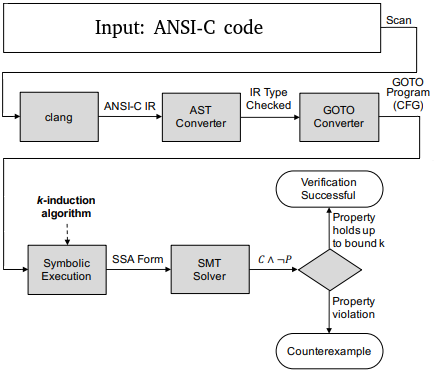
\includegraphics[width=0.4\textwidth]{ESBMCarch4}
%\centering
%\caption{ESBMC architecture (adapted from \cite{esbmc2018}).}
%\label{fig:esbmcarch}
%\end{figure}
%ESBMC uses clang as front-end, a state-of-the-art compiler suite for C/C++/ObjectiveC/ObjectiveC++ widely used in industry \cite{esbmc2018}. % and generate an Abstract Syntax Tree (AST). %%%%%One legacy CBMC-based front-end that supports both C and C++ and a new clang-based front-end that currently only supports C. The data types and bit vectors are created in the front-end when parsing the code. 
%%%%%%%Regardless of the chosen front-end, 
%The output is an AST (tree representation of the abstract syntactic structure of source code written in a programming language) that will be used by the GOTO converter to generate a GOTO program, which has simplified control flow and is suitable for bounded unwinding. The next step is the symbolic execution, when the GOTO program is executed (unrolling loops up to the bound $ k $) and converted to Static Single Assignments (SSA) form. SSA form enables the simplification of algorithms and reduction of computational complexity. %%%%%%%%%, where each variable is a target of exactly one assignment statement in the program text. 
%The feature called k-induction at Fig. \ref{fig:esbmcarch} allows the model checker to find a property violation or even to prove (partial) correctness without fully unwinding loops. 
%%
%%%%%%%During the symbolic execution, ESBMC aggressively tries to simplify the program \cite{Ramalho}; it propagates all constants and solves any assertions that can be statically determined. This is an important step for the verification, since ESBMC can fully verify programs without calling a solver, if the inputs are deterministic. That characteristic is useful at this work to perform the sizing check of the PV system project. 
%Following, the SSA expressions are then encoded using the chosen SMT solver supported by ESBMC. At this paper, it was used the Z3 solver \cite{DeMoura}.
%%%%%: Boolector (default) \cite{Brummayer}, Z3 \cite{DeMoura}, MathSAT \cite{Cimatti}, Yices \cite{Dutertre} and CVC4 \cite{Barrett}. 
%
%Finally, the system attempting to determine whether a formula, which is the disjunction of all possible errors, can be satisfied. 
If the SMT formula is shown to be satisfiable (SAT), a counterexample is presented; otherwise, the formula is unsatisfiable (UNSAT), i.e., there are no errors up to the given unwinding bound. 

% incremental ESBMC text here
ESBMC exploits the standardized input language of SMT solvers (SMT-LIB\footnote{http://smtlib.cs.uiowa.edu/} logic format) to make use of a resource called \textit{assertion stack}. An assertion, in SMT solvers, is a constraint over the variables in a formula that must hold if the formula is satisfiable~\cite{Morse2015}. New assertions can be added to or old assertions removed from this stack, depending on the evaluated value of variables. This enables ESBMC, and the respective solver, to learn from previous checks, optimizing the search procedure and potentially eliminating a large amount of formula state space to be searched, because it solves and disregards data during the process, incrementally. This technique is called 'incremental SMT'~\cite{DBLP:journals/fac/SchrammelKBMTB17} and allows us to reduce the memory overhead, mainly when the verified system is complex and the computing platform does not have large amount of memory to deal with all the design space state.
\subsection{Ultimate Automizer}
%Ultimate Automizer is an automatic software verification tool for C programs. This tool is the first implementation of trace abstraction, which is an automata-theoretic approach to software verification. The implemented algorithm uses nested interpolants in its interprocedural program analysis.
Ultimate Automizer is an automatic software verification tool for C programs that is able to check safety and liveness properties. The tool implements an automata-based instance of the CEGAR scheme. CEGAR or Counterexample-Guides Abstraction Refinement is a technique that iteratively refines an abstract model using counterexamples and use three concepts: precision, feasibility check, and refinement~\cite{CEGAR}.
%(i) precision, for the level of abstraction; (ii) feasibility check, deciding if there is a concrete error path; and (iii) a refinement procedure, which takes as input as infeasible error path and extracts a precision that suffices to instruct the exploration algorithm do not explore the same path again later~\cite{CEGAR}.

In each iteration, Automizer pick a trace (sequence of statements) that leads from the initial location to the error location and check whether the trace is feasible or infeasible. If the trace is feasible, an error is reported to the user; otherwise it is computed a sequence of predicates along the trace as a proof of the trace’s infeasibility. The predicates are a sequence of interpolants since each predicate “interpolates” between the set of reachable states and the set of states from which we cannot reach the error. In the refinement step of the CEGAR loop, Automizer tries to find all traces whose infeasibility can be shown with the given predicates and subtract these traces from the set of (potentially spurious) error traces that have not yet been analyzed. It is used automata to represent sets of traces. The difference to a classical CEGAR-based predicate abstraction is that Automizer have to do any logical reasoning (e.g., SMT solver calls) that involves predicates of different CEGAR iterations~\cite{Automizer2018}. 
%
%----------------------------------------
\section{Automated verification of Stand-alone Solar PV Systems }
\label{sec:Methodology}
%----------------------------------------
\subsection{Stand-alone Solar PV Systems}
PV systems are classified into distinct types~\cite{Mohanty}. Specifically for remote rural areas of developing countries or places where the grid extension is not feasible, the most suitable configuration is the regulated stand-alone system with battery and AC load; this configuration is the focus of case-studies of this work.

The mathematical modeling of the PV system is based on modular blocks, as illustrated in Fig.\ref{fig:blockdiagram}. It identifies the PV generator, batteries, charge controller, inverter, and AC load. The PV generator, which can be a panel or an array, is a semiconductor device that can convert solar energy into DC electricity. In Fig.\ref{fig:blockdiagram}, there are two variables that depend on the site where the system is deployed and the weather (i.e., solar irradiance $G$ and temperature $T$). For night hours or rainy days, we need to hold batteries, where power can be stored and used. The use of battery as a storage form implies the presence of a charge controller~\cite{Hansen}. The PV arrays produce DC and therefore when the PV system contains an AC load, a DC/AC conversion is required. That converter is called of inverter; and the AC load dictates the behavior of AC electrical load from the house that will be fed by the system.
\begin{figure}[h]
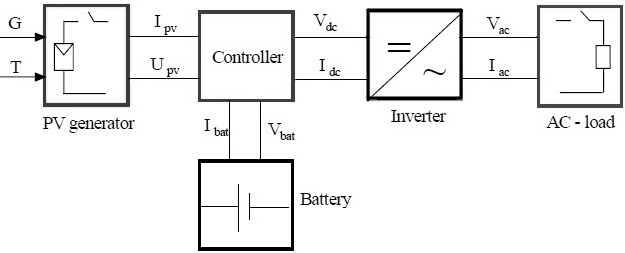
\includegraphics[width=0.6\textwidth]{blockdiagramPVS2}
\centering
\caption{Block diagram for a typical stand-alone PV system~\cite{Hansen}.}
\label{fig:blockdiagram} 
\end{figure}
A wide variety of models exists for estimation of power output of PV modules (and $I-V$ or $P-V$ curves). However, the present work will rely on the simplified model of 1-diode. It was demonstrated that it has a small error rate, between 0.03\% and 4.68\% from selected PV panels tested~\cite{Saloux}. The model uses formulas from different references~\cite{Hansen}, \cite{Saloux}, and \cite{Ross}.

To model the batteries, it was used the most common based on lead-acid~\cite{Copetti}. Related to the charge controller, it was used the 4-steps controller processes with MPPT (maximum power point tracking) to decide if the PV array must be disconnected from the system, or if the PV can be reconnected, or if the load is disconnected and when the load is reconnected~\cite{Hansen}. The inverter model is the simplest and is based on efficiency, i.e., the relation between the AC output power and the DC input power of the component~\cite{Hansen}. The AC load, from every case study, is defined by a 24 hour curve who reflects the estimated use of all electrical loads from the house. Load information was collected during a presential survey performed in each house.

\subsection{Automated Verification Methodology}
In order to evaluate the automated tools when verifying stand-alone solar photovoltaic systems, we created a methodology where each tool will process the ANSI-C code with constraints %($C$) 
and properties %($P$) 
from the PV system that are provided by the user, and the tool will automatically verify if the PV system requirements are met. If it returns a failure (i.e., SAT), then the tool provides a counterexample, i.e., a sequence of states that leads to the property violation. However, if the verification succeeds (i.e., UNSAT), there is no failure up to the bound $k$; therefore, the PV system will present its intended behavior up to the bound $k$.

The methodology can be described as a three stage process. In Step 1, the PV input data (e.g., load power demand and load energy consumption) and the formulae to check the sizing project, the mathematical model, the limits of the weather non-deterministic variables, are all written as an ANSI-C code~\cite{ANSI2018}. In Step 2, the sizing check of the PV system takes place to make sure that the components were selected according to critical month method~\cite{Pinho}. %%%The equations to check the PV sizing were not presented at this paper, however the standard from Engineering Manual was the reference~\cite{Pinho}.
%
In Step 3, weather variables (e.g., solar irradiance and ambient temperature) will be systematically explored by our verification engine based on maximum and minimum values from the site, where the PV system will be deployed. 
%As a consequence, all the formulae of the employed mathematical models will also be updated. 
In addition, depending on one of the desired properties of the system such as battery autonomy, energy availability, or even system power supply, our verification engine is able to indicate a failure if those properties are not met; in this particular case, it provides a diagnostic counterexample that shows in which conditions the property violation occurred. 
%; as the  state of charge of the batteries, load demand of power and the load consumption of energy if defined by the code
% (as reliability, performance, or safety)
%
%\textcolor{red}{In the following paragraph you should related the output of our verification engine with the description of the BMC SAT or UNSAR given above. For example, what does a failure mean? is it SAT?}
%, i.e., our verification engine does not give any guarantee that there is no error in bound $k+1$ unless some induction method is employed~\cite{DBLP:journals/sttt/GadelhaIC17}.
%
%
%---------------------------------------------------------------------
% \subsection{The case studies and the Algorithm}
%---------------------------------------------------------------------
%
% 
%and as backup at night 
%
%The 700 W system: 3 x 325 W PV panels connected in series, controller of 150 V/35 A with a DC-bus of 24 V, 4 x 220 Ah batteries (2 in series and 2 in parallel arrangement), and inverter of 700 W. 
%
%And the 1,200 W PV system: 4 x 325 W connected in series PV panels, with controller of 150 V/35 A  in a DC-bus of 48 V, 4 batteries of 120 Ah connected in series, and a 1,200 W inverter.
%
%As demonstrated at this work, the performance of the system is highly dependent of solar irradiance and temperature, that are specific of the deployed local (latitude and longitude). 

Algorithm~\ref{alg:verification-algorithm} describes the pseudo-code used to perform the automated verification. %Line 1 indicates a function call that performs the size checking of the each component of the PV system. %: using Equations \eqref{eq:NTPmin}, \eqref{eq:NTP}, \eqref{eq:NPSmin}, \eqref{eq:NPS}, \eqref{eq:NPP}, and \eqref{eq:NPPmin} to verify the PV panel; using \eqref{eq:Cbank}, \eqref{eq:Nbtotal}, and \eqref{eq:batcheck} to verify the batteries; using \eqref{eq:vcvsystem}, \eqref{eq:icmin}, and \eqref{eq:icicmin} to verify the charge controller; and using \eqref{eq:vindc}, \eqref{eq:voutac}, and \eqref{eq:invcheck} to verify the inverter. 
%The verification is carried out by the \textit{assert} macro from the ANSI-C programming language to encode each equation of sizing check. The argument to the \textit{assert} statement must be \textit{true} if the system specification is met; otherwise, the program aborts and prints a counterexample indicating a property violation. If there is no property violation, then the verification algorithm continues and 
The batteries are assumed to have initial SOC of 80\% (Line 1). %%100% before, i.e., the batteries are charged. That is important because the system is said ready to use when the batteries are charged.
%At both case studies, it was considered 21 years of historic data from Manaus. 
%According with X and Y, t
Information related to average temperature ($T$) and solar irradiance ($G$), maximum and minimum annual, are given to the algorithm in Lines 7 to 10 using non-deterministic variables from ESBMC to explore all possible states and the \textit{assume} macro to constrain the non-deterministic values using a given range. 
%and irradiance varies from 0 W/m$^{2}$ to 852 W/m$^{2}$ (with minimum of 274 W/m$^{2}$ during the daytime, when there is sunlight). 
%there is PV generation only between 8:00 h and 16:00 h every day, 
%with zero electric energy generation from 18:00 h to 6:00 h of the next day; and with insignificant generation from 6:00 h to 8:00 h, and from 16:00 h to 18:00 h of the same day. 
In order to reduce the computational effort of the algorithm,
% caused by the state explosion inherent of the technique, 
every 24h-day was considered as a time-step of 1 hour, and it was split into two parts: (a) one where it is possible to occur PV generation, during daylight, with a duration in hours depending on each site (but dependent on the sun and weather conditions); and (b) one that includes all the remaining day (without any PV generation). Therefore, our approach depends on specific data about the solar irradiation levels to define the average amount of hours of PV generation.

After that, the model from PV generator is used in the function call of Line 7, to produce the voltage and current considering the states of $G$ and $T$. With respect to every hour considered, the conditional \textit{if-else-endif} statements from Lines 8, 11, 13, 16 and 19, will perform the charge or discharge of batteries according to the value of different variables: if there is PV generation (which depends on $G$ and $T$), the updated state of charge from batteries, the house's load and the set-up information of the PV system.

Next, representing the time of the day where PV generation is not possible anymore, starting in Line 22, the algorithm will only discharge the batteries (using the 1 hour step) until a new charging process (at the next day) starts. Specific \textit{assert} in Line 26 will check the state of charging from batteries, and they will violate the property if their levels reach the minimum that represents a discharged battery; therefore, the PV system is unable to supply energy to the house. Nevertheless, if the verification engine does not fail, then we can conclude that the PV system does not need further corrections up to the given bounds.
%
%\textcolor{red}{this sentence is unclear... After this process is started the battery autonomy verification, from line 31}. \textcolor{red}{this sentence is unclear... Based on the fact that won't be PV generation after a given time of the day, the algorithm will only discharge the batteries until a new charging process (at the next day) to start.} \textcolor{red}{what do you mean by The formal verification is guaranteed?...  The formal verification is guaranteed by  macro to specific variables of the model, according lines 27 and 35.}
% and the non-deterministic variables $G$ and $T$ are considered during the formal verification of the system, otherwise, during the other two periods, there is no PV generation and just the power consumption from the backup batteries. 
%Within this 8h-period, $G$ and $T$ are automated verified with different values every one hour.
%, and change their value every 1 h according with the algorithm created using the technique.
 \begin{algorithm}
 \caption{Model checking algorithm for stand-alone PV}
 \begin{algorithmic}[1]
 \renewcommand{\algorithmicrequire}{\textbf{Input:}}
 \renewcommand{\algorithmicensure}{\textbf{Output:}}
  \STATE $SOC \leftarrow 80\%$ \\
%  \COMMENT {Starting with the PV generation time}
% \\ 
 \textit{LOOP Process}
  \FOR {$h = 1$ to $Hours \, of \, PV \, generation$}
  \STATE $G \leftarrow nondet \textunderscore uint(\,)$ \COMMENT {$G$ is non-deterministic variable}
  \STATE $T \leftarrow nondet \textunderscore uint(\,)$ \COMMENT {$T$ is non-deterministic variable}
  \STATE assume ($Gmin \leq G \leq Gmax$) \COMMENT {restricting $G$ values}
  \STATE assume ($Tmin \leq T \leq Tmax$) \COMMENT {restricting $T$ values}
  \STATE $Imax, Vmax \leftarrow PVgenerationMODEL (G,T)$ 
  \\
%  \COMMENT {If-then-else sequence to imitate charge controller work}
  \IF {($battery \, is \, empty$) AND ($PV \, is \, generating$)}
    \STATE charge battery in 1h
    \STATE PV feed the house
  \ELSIF {($battery \, is \, empty$) AND NOT($PV \, is \, generating$)}
    \STATE FAIL with assert macro
  \ELSIF {NOT($battery \, is \, empty$) AND ($PV \, is \, generating$)}
    \STATE stop battery charge
    \STATE PV feed the house
  \ELSIF {NOT($battery \, is \, empty$) AND NOT($PV \, is \, generating$)}
    \STATE discharge battery in 1h
    \STATE Battery feed the house
  \ENDIF
  \STATE $h \leftarrow (h+1)$
  \ENDFOR
 \\ \textit{Start of battery autonomy verification:}
%%  initialization\;
\STATE $AutonomyCount \leftarrow 1$
 \WHILE {$AutonomyCount \leq autonomy$}
  %%\FOR {$Autonomy = 1$ to $auton$}

  \STATE $SOC \leftarrow SOC - ( 24 - Hours \, of \, PV \, generation)\,h\, discharge$
  \STATE $AutonomyCount \leftarrow AutonomyCount+1)$
  \\  
%    \COMMENT {autonomy verification during discharge period}
%  \\
  \STATE assert NOT($Battery \, empty$)  
  \\
  \COMMENT {Perform similar \textbf{for}-LOOP as defined in line 2-21}
  %%\ENDFOR
  \ENDWHILE
 \RETURN $(\,)$ 
 \end{algorithmic} 
 \label{alg:verification-algorithm}
 \end{algorithm}

\section{Experimental Evaluation} 
\label{sec:results}
%------------------------------------------
\subsection{Description of the Case Studies}
%------------------------------------------
We have performed five case studies to evaluate the tools: (a) four PV systems (three in series 325W PV panels, four 220 Ah batteries in a configuration with two series and two parallel with 48h autonomy, 700 W inverter with surge of 1,600W, charge controller with MPPT with 35A/150V of capacity) deployed in four different houses in an indigenous community (GPS coordinates 2$^{o}$44'50.0"S 60$^{o}$25'47.8"W) situated nearby Manaus (Brazil), with each house having a different power demand (house 1 = 253 W, house 2 = 263 W, house 3 = 283 W, and house 4 = 501 W); and (b) one case concerning a system deployed as an individual system in Manaus (GPS coordinates 3$^{o}$4'20.208"S 60$^{o}$0'30.168"W), supporting 915 W of the house's load (house 5 with four 325W PV panels in a configuration two series and two parallel, four 120Ah batteries in series and autonomy of just 6 h, 1,200 W inverter with surge of 1,600 W, charge controller with MPPT of 150V/35A). 

The annual average temperature ($T$) in Manaus is from 23$^{o}$C to 32$^{o}$C; and irradiance ($G$) varies from 274 W/m$^{2}$ to 852 W/m$^{2}$ when there is sunlight (that information is provided in Lines 5 and 6 of Algorithm~\ref{alg:verification-algorithm}). Another characteristic of Manaus, based on historical weather data %\cite{Temperature}, 
\cite{Irradiance}, is related to the fact that only during 8 hours of the day is possible to have PV generation, from 8:00h to 16:00h (that information is provided in Algorithm~\ref{alg:verification-algorithm} as well).

%------------------------------------------
\subsection{Objectives and Setup}
%------------------------------------------
Our experimental evaluation aims to answer two research questions:
%
\begin{enumerate}
\item[RQ1] \textbf{(soundness)} Does the automated verification provide correct results?
\item[RQ2] \textbf{(performance)} How does the  tools compare each other?
\end{enumerate}

It was used two different setups of hardware and different verification engines, combined with different Solvers. The aim was to evaluate different environments and possible user limitation in terms of main processor and RAM memory. All the experiments were performed without a predefined timeout.

Mostly of experiments were conducted on an otherwise idle Intel octa core Xeon CPU E5-2640 with 2.4 GHz and 264 GB of RAM, running Ubuntu 18.04.1 LTS 64-bits. It was called high-end setup and the verification engines demanded around 90G bytes of RAM (each process).

In addition, it was considered a low-end setup, using specifically the incremental option of ESBMC verification engine, where the demand of memory is very low (2G Bytes of RAM). The experiments were conducted on an otherwise idle Intel Core i7-2600 (8-cores), with 3.4 GHz and 32 GB of RAM, running Ubuntu 18.04.1 LTS 64-bits. 

Concerning the high-end configuration: (i) verification engine ESBMC, version v5.1.0 was used with the SMT solver Boolector version 2.4.1~\cite{Brummayer}\footnote{The command-line used to perform verification: \$ esbmc filename.c -\phantom{}-no-bounds-check -\phantom{}-no-pointer-check -\phantom{}-no-div-by-zero-check -\phantom{}-unwind 300 -\phantom{}-boolector}; (ii) verification engine CBMC 5.6 and MiniSat~\cite{Kroening}\footnote{The command-line used to perform verification: \$ cbmc filename.c --unwind 300}; (iii) Ultimate Automizer version 0.1.24~\cite{Automizer2018}\footnote{The command-line used to perform verification: \$ ./Ultimate -tc config/AutomizerReach.xml -i filename.c}.
 
% enabled with the goal of reducing memory usage; 
%The experiments were performed without a predefined timeout.
Concerning the low-end configuration: ESBMC v5.1 was used with the SMT incremental mode\footnote{The command-line used to perform the verification is: \$ esbmc filename.c -\phantom{}-no-bounds-check -\phantom{}-no-pointer-check -\phantom{}-no-div-by-zero-check -\phantom{}-unwind 300 -\phantom{}-smt-during-symex -\phantom{}-smt-symex-guard -\phantom{}-z3} enabled with the goal of reducing memory usage; we have also used the SMT solver Z3 version 4.7.1~\cite{DeMoura}. 

In order to evaluate the verification methods and its performance, we have considered five case studies and also compared its performance to the HOMER Pro tool. %Every dweller, who owns a PV system, was interviewed to get information about his/her PV system during four months of use. This information was used to know possible flaws from every system in the field.
Experimental setup of HOMER Pro: Intel Core i5-4210 (4-cores), with 1.7 GHz and 4 GB of RAM, running Microsoft Windows 10; we have used HOMER Pro v3.12.0. 

%------------------------------------------
\subsection{Results}
\label{sec:results_indeed}
%------------------------------------------
%
The Table~\ref{tab1} summarize the results concerning the use of the automated verification tools applied to the five case-studies of a solar PV system.

\begin{table}
\centering
\caption{Summary of the case-studies comparative and the automated tools.}\label{tab1}
\begin{tabular}{|c|c|c|c|c|}
\hline
\hline
\multicolumn{5}{|c|}{Model Checker (SAT/UNSAT: time and message)}\\
\hline
Case &  \makecell{ESBMC \\(Boolector)} & \makecell{CBMC\\(MiniSat)} & UAutomizer & \makecell{ESBMC Incremental\\(Z3)}\\
\hline
\hline
House 1 &  \makecell{7.44h \\(low SOC after 16:00h)} & \makecell{Inconclusive \\(during solver)} & XX & \makecell{409.3h \\ (low SOC after 16:00h)}\\
\hline
House 2 &  \makecell{5.74h \\(low SOC after 16:00h)} & \makecell{Inconclusive \\(during solver)} & XX & \makecell{611.2h \\ (low SOC after 16:00h)}\\
\hline
House 3 & \makecell{Inconclusive \\(during solver)} & \makecell{Inconclusive \\(during solver)} & XX & \makecell{615.8h \\ (low SOC after 16:00h)}\\
\hline
House 4 & \makecell{5.52h \\(low SOC after 16:00h)} & \makecell{Inconclusive \\(during solver)} & XX & \makecell{620.8h \\ (low SOC after 16:00h)}\\
\hline
House 5 & \makecell{0.55h \\(Sizing: number of panels)} & \makecell{Inconclusive \\(during solver)} & XX & \makecell{63.3h \\ (Sizing: number of panels)}\\
\hline
\hline
\end{tabular}
\end{table}

\section{Conclusions and Future Work}
We have described and evaluated different automated verification methods to check whether a given PV system meets its specification using software model checking techniques. We have considered five case studies from real photovoltaic systems deployed in five different sites, ranging from $700$ W to $1,200$ W. ESBMC had the better results, in both setups (high-end and low-end configurations). Although the verification method takes longer than simulation methods, it is able to find specific conditions that lead to failures in a PV system previously validated by a commercial simulation tool. In particular, the proposed method was successful in finding sizing errors and indicating in which conditions a PV system can fail. Future work will focus in other verification engines and different solvers, besides the improvement of the algorithm in order to obtain better performance.
%
% ---- Bibliography ----
%
% BibTeX users should specify bibliography style 'splncs04'.
% References will then be sorted and formatted in the correct style.
%
\bibliographystyle{splncs04}
\bibliography{trindadeThesis}
%

\end{document}

%\subsection{Design and Simulation of Solar PV systems}
%The design and validation of a PV system can be done by hand or with the aid of a software tool. In order to address different aspects of the PV system design, there are various software tools available in the literature~\cite{Rajanna,Rawat}.
%public domain and commercial software available for the PV market. 
%According to \cite{Brooks}, t
%%%%%%%%%%
%
%The capabilities of tools available in the literature range from simple solar resource and %energy production estimation, %to site survey and system design tools,
%to complex financial analysis and project optimization. At this study, the commercial simulation tool HOMER PRO was selected to be used at the case studies in order to be compared with the automated verification tools.
